%%%%%%%%%%%%%%%%%%%%%%%%%%%%%%%%%%%%%%%%%
% MPhys Report
% Semester 2
% 
% Started on 04/05/16
% Author: Rhiannon Jones
% 4th Year MPhys Sem2
% 
%%%%%%%%%%%%%%%%%%%%%%%%%%%%%%%%%%%%%%%%%

%----------------------------------------------------------------------------------------
%	PACKAGES AND OTHER DOCUMENT CONFIGURATIONS
% Downloads the required packages for certain features
%----------------------------------------------------------------------------------------

\documentclass[11pt]{article}
\usepackage[utf8]{inputenc}
\usepackage{amsmath}
%\usepackage{amsfonts}
\usepackage[sc]{mathpazo}
\linespread{1.05}         % Palladio needs more leading (space between lines)
\usepackage[T1]{fontenc}
%\renewcommand*\rmdefault{Type1}
\usepackage{ulem}
\usepackage{amssymb}
\usepackage{verbatim}
\usepackage{graphicx}
\usepackage{courier}
\usepackage{cite}
\linespread{1.2} % Line spacing - Palatino needs more space between lines
% Load all packages needed for all sub−files:
\usepackage{xcolor}
\definecolor{purpleX}{rgb}{0.573,0,1}
\definecolor{greenX}{rgb}{0.349,0.831,0.329}
\usepackage{geometry}
 \geometry{
 a4paper,
 total={210mm,297mm},
 left=28mm,
 right=28mm,
 top=30mm,
 bottom=30mm,
 }% Document margins
\usepackage{multicol} % Used for the two-column layout of the document
\usepackage{color}
\setlength{\columnseprule}{1pt}
\def\columnseprulecolor{\color{gray}}
\usepackage[hang, small,labelfont=bf,up,textfont=it,up]{caption} % Custom captions under/above floats in tables or figures
\usepackage{booktabs} % Horizontal rules in tables
\usepackage{float} % Required for tables and figures in the multi-column environment - they need to be placed in specific locations with the [H] (e.g. \begin{table}[H])
\usepackage{paralist} % Used for the compactitem environment which makes bullet points with less space between them
\usepackage{abstract} % Allows abstract customization
\renewcommand{\abstractnamefont}{\LARGE} % Set the "Abstract" text to bold
\renewcommand{\abstracttextfont}{\itshape} % Set the abstract itself to italic text
\usepackage{titlesec} % Allows customization of titles
\titleformat{\section}[block]{\large}{\thesection.}{.8em}{} % Change the look of the section titles
\titleformat{\subsection}[block]{\scshape\itshape}{\thesubsection.}{.8em}{} % Change the look of the section titles

%----------------------------------------------------------------------------------------
%	TITLE SECTION
%----------------------------------------------------------------------------------------

\title{\vspace{5mm}\fontsize{20pt}{12pt}\selectfont A preliminary investigation into determining \\ \vspace{3mm} CC0\(\pi\) cross-section sensitivities in SBND \\ } % Article title

\author{
    \date{}
}

%----------------------------------------------------------------------------------------

\begin{document}

\nocite{*}

\pagenumbering{gobble}

\maketitle % Insert title

\vspace{-9mm}

\begin{figure}[h!]
    \center
    
\includegraphics[scale=0.6]{images/UoL_CoA.pdf}
\end{figure}

\vspace{3mm}

\begin{center}

    \large Rhiannon Jones\\
    \normalsize University of Liverpool \\
    \normalsize School of Physical Sciences \\ % Institution
    \normalsize rjones@hep.ph.liv.ac.uk \\ 
    \vspace{3mm}
    \normalsize 1\( ^{ \mbox{\footnotesize st } } \) year PhD report \\

\end{center}

\vspace{6mm}
%----------------------------------------------------------------------------------------
%	ABSTRACT
%----------------------------------------------------------------------------------------
\begin{abstract}
    Random stuff
\end{abstract}
\newpage
%----------------------------------------------------------------------------------------
%	ARTICLE CONTENTS
%----------------------------------------------------------------------------------------
\pagenumbering{arabic}
\section{Introduction}
\label{sec:intro}

Neutrino physics is at the core of current high energy research. One of the profound discoveries made in recent years was the observation of neutrino flavour oscillations by the Super-Kamiokande (Super-K) experiment, which was the first confirmation that physics existed beyond the standard model of particle physics. In brief, neutrinos described by the standard model would be massless particles, but since the flavours are made up of superpositions of mass states, the oscillation of
the flavour states implies that the relative mass states are different, and therefore non-zero \cite{nuInt}.

    Future, long-baseline,  neutrino experiments such as the Deep Underground Neutrino Experiment (DUNE) and Hyper-Kamiokande (Hyper-K) are hoping to investigate some of the most fundamental questions we are still asking: Why does the universe constist of matter, and not anti-matter? What is the neutrino mass heirarchy? Neutrino research is an extremely active field. Optimising the current and future detectors to maximise the accuracy of all interaction anaylses is a crucial step towards obtaining concrete answers to these questions. 

    A brief introduction to the topics covered in this report is as follows, more detail on each will be given in later sections. 

\subsection{Neutrino interactions}

Due to the elusive nature of the neutrino, directly observing one in a detector isn't possible. It is therefore necessary to infer their existence from particles produced when they interact. Since this process relies upon the reconstruction capability of the experiment, purpose-built detectors will attempt to maximise the efficiency of this.

Another property of the neutrino which poses a significant difficulty within detectors is their interaction probability, or cross-section. A typical neutrino cross-section is on the order of $ 10^{-44} $ cm$^{2}$ which corresponds to $\sim$1 interaction every 10 light years in steel, for neutrinos with only a few MeV energy \cite{nuOsc}. This fact introduces the need for the interacting neutrinos to have high energies in these dedicated experiments, if we are to sufficiently reduce their mean free path. More detail on this topic will be discussed in section~\ref{sec:NIP}.

\subsection{GENIE and the GENIE-Professor global fits}

GENIE is the world leading Monte Carlo neutrino interaction generator. Generators are a crucial machinery in all high energy physics analyses as they use theoretical models to produce predictions of how and where neutrino interactions will occur in specific detector geometries \cite{genie}. With this information, comparisons between experimental data and theoretical predictions can be drawn, the models can be improved through fits to such data and potential new physics can be explored. These predictions also help motivate the requirements for building state-of-the art detectors and produce high precision cross-section measurements to improve current and future neutrino physics analyses. 

    An effort to improve model configurations by performing fits to an archive of experimental data is currently being carried out by GENIE using the Professor software framework, which was written with this purpose for experiments at the LHC \cite{prof}. The ultimate goal of this exercise is to perfom a global fit to all neutrino scattering data and consequently produce comprehensive model configurations to further optimise the predictions made for the next generation of neutrino experiments. This work and GENIE's role in current and future neutrino experiments will be discussed further in section~\ref{sec:GF}.

\subsection{Cross-sections}
   
    In order to correctly model neutrino events within a specific detector geometry and material, certain parameters have to be known. In particular, the probability of an interaction taking place - its cross-section - is required for each possible interaction the neutrino could undergo. Cross-section measurements are therefore a necessity for the Monte Carlo event generators, and consequently the future detector studies mentioned earlier. 
    
    The extent of our current knowledge of charged current neutrino cross sections is shown in Figure~\ref{fig:xsecCurr}. The plot contains cross-section information from multiple types of neutrino experiment, differing in both target material and detector machinery. A feature of this plot which is of the most interest to a Short Baseline Near Detector (SBND) cross-section study in particular, is the lack of precision in the measurements made towards the $\sim$1 GeV region
    \cite{xsecCurr}. SBND will not only be operational at this energy range, but it will also have statistics substantial enough to potentially make a significant contribution to improving the current knowledge in this region.

    %CC cross-sections
    \begin{figure}[h!]
        \center
        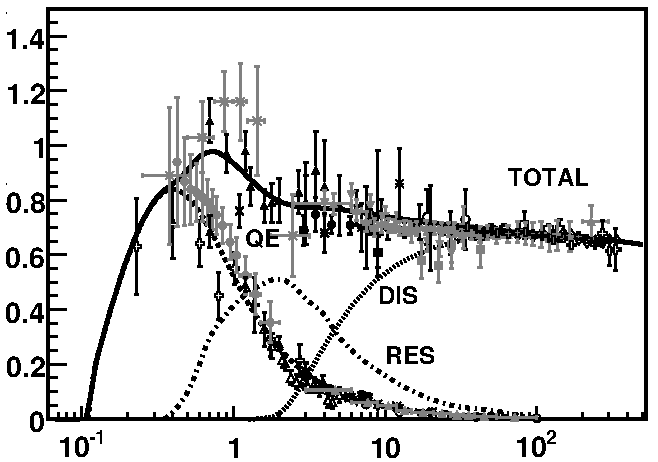
\includegraphics[width=.8\textwidth]{images/current_cross_sec_knowledge.pdf}
        \put(-68, -15){\Large E$_{\nu}$ ( GeV )}
        \put(-375, 50){\Large \rotatebox{90}{$\sigma_{\nu}$ / $\Delta$E$_{\nu}$ ( 10$^{-38}$ cm$^{2}$ / GeV ) }}
        \caption{A compilation of the total cross-section data across the $\sim$1 MeV to $\sim$100 GeV energy range. Including a breakdown in terms of the quasi-elastic, QE, resonant, RES and deep inelastic scattering, DIS, topologies \cite{xsecCurr}. }
        \label{fig:xsecCurr}
    \end{figure}

    The scale of contribution SBND could make to this area of physics would in turn improve the predictions made by event generators for the next generation of neutrino experiments. Cross-sections will be discussed further in section~\ref{sec:XSec}.
    
\subsection{SBND Physics Goals}

SBND is one of 3 liquid argon detectors using the same neutrino beam in the Short Baseline Neutrino (SBN) program. Together, they aim to explore neutrino oscillations at 3 different positions along the beam, allowing for highly senstive measurements to be made \cite{sbn}.   

Another objective of the SBN program, along with many other neutrino physics experiments, is to observe or reject the existence of sterile neutrinos. Though this will not be discussed here.

The MiniBooNE and LSND experiments observed an excess of low energy electron neutrino appearance in their data \cite{mbEx}. One of the main physics goals of SBND is to look for and characterise this excess, in collaboration with any results obtained by the MicroBooNE experiment before SBND is taking data. The beamline of MicroBooNE is 470m compared to 110m for SBND, whether one or both experiments observe the excess will tell us if there was a dependence on the distance travelled by the neutrinos \cite{sbn}. \\

This report will further describe the current status of neutrino cross-section analyses, the level importance that these measurements have in the field, and how a sensitivity calculation in the low GeV energy region is being carried out. It will then explain in more detail how Monte Carlo neutrino generators can be, and are being improved using recent and historical scattering data, through a global fit of comprehensive theoretical model configurations.  

\clearpage


%---------------------------------------------------------------------------------------------------------------
\section{Neutrino Interaction Phenomenology in the few-GeV Energy Range}
\label{sec:NIP}

\subsection{Dominant topologies}

The statistics given in Figure~\ref{fig:sbndStats} indicate that the dominant interactions observable in SBND will be CC0$\pi$ and CC1$\pi ^{\pm}$, example Feynman diagrams of the main contributing processes at the free-nucleon level are given in Figure~\ref{fig:feyn}. 

    \begin{figure}[h!]
        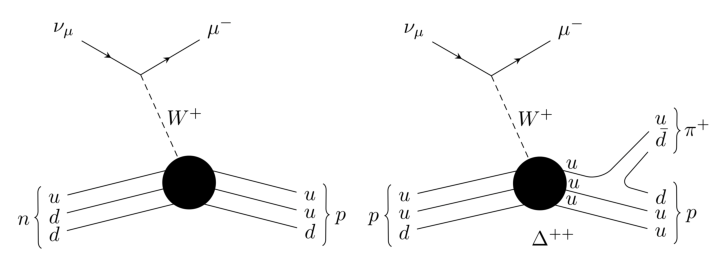
\includegraphics[width=\textwidth]{images/feynmans.pdf}
        \caption{On the left-hand side is a Feynman diagram of the CCQE interaction. During this process, the incoming neutrino interacts with a neutron and produces a muon and a single proton as the observable final state particles. On the right is the postive version of the CC1$\pi ^{\pm}$ interaction, in which a neutrino interacts with a proton emitting a $\pi ^{+}$ alongside the final state muon and proton. Here, the invariant mass of the entire hadronic system must be accounted for when reconstructing the neutrino energy.}
        \label{fig:feyn}
    \end{figure}

One dominant background to the CC0\(\pi\) process is an NC1\(\pi^{\pm}\) interaction, in which the final state pion may decay rapidly into a muon leaving the appearance of a single proton and muon final state as described in equations~(\ref{eq:NC1pi}).

    \begin{equation}
        p + \nu_{\mu} \longrightarrow \nu_{\mu} + p + \pi^{-}
    \end{equation}
    \begin{equation}\label{eq:NC1pi}
        \downarrow
    \end{equation}
    \begin{equation}
        \pi^{-} \longrightarrow \mu^{-} + \bar{\nu}_{\mu}
    \end{equation}

    Backgrounds such as this are an important consideration in all analyses. Though in high resolution detectors such as SBND, the ability to distinguish true signal should be possible to the extent that impurity contributions are minimal. 

\subsection{Energy reconstruction}

    The energy of the incoming neutrino must be reconstructed from the other particles involved in the interaction. When dealing simply with a 2-body hadronic process, such as the one shown in the left hand side of Figure~\ref{fig:feyn}, it is acceptible to use the quasi-elastic estimation~(\ref{eq:Ereco}) \cite{teppei} to calculate the reconstructed energy, $\bar{E}_{\nu}$. Where $E_{\mu}, m_{\mu}$ and $\underline{k}'_{\mu}$ are the energy, mass and 3-momentum of the final state
    muon, $M_{N}$ is the mass of a target nucleon and $\theta$ is the opening angle between the outgoing muon and proton \cite{teppei}.  


    \begin{equation}\label{eq:Ereco}
        \bar{E}_{\nu} = \frac{ E_{\mu} - m^{2}_{\mu} / (2M_{N}) }{ 1 - ( E_{\mu} - |\underline{k}'_{\mu}| cos \theta ) / M_{N} }
    \end{equation}

Alternatively, if the interaction involves more particles in the final state, such as multiple protons or pions escaping the nucleus, one must account for the energy given to all of the hadronic final state particles in the energy reconstruction. 

\subsection{Complications in the free nucleon theory}

Theoretical models of physical interactions on free nucleons are well-grounded, since any incoming particles will interact entirely externally to the particles they collide with. However, when dealing with nuclear targets in high energy physics experiments, such as SBND, complications occur in our understanding of the true nature of the interactions taken place, and data can become inexplicable in comparison with models built on free nucleon cross sections \cite{dipReg}. 

For instance, in the few-GeV energy range, neutrinos will be able to penetrate the argon nucleus and interact with individual nucleons. Therefore, an observation of the CC0\(\pi\) interaction in SBND would not necessarily indicate that a CCQE process took place between the neutrino and nucleon. Pions may be produced initially but be absorbed before ever escaping, thus leaving them invisible to the detector, this is visualised in Figure~\ref{fig:interNuc}.

    \begin{figure}[h!]
        \centering
        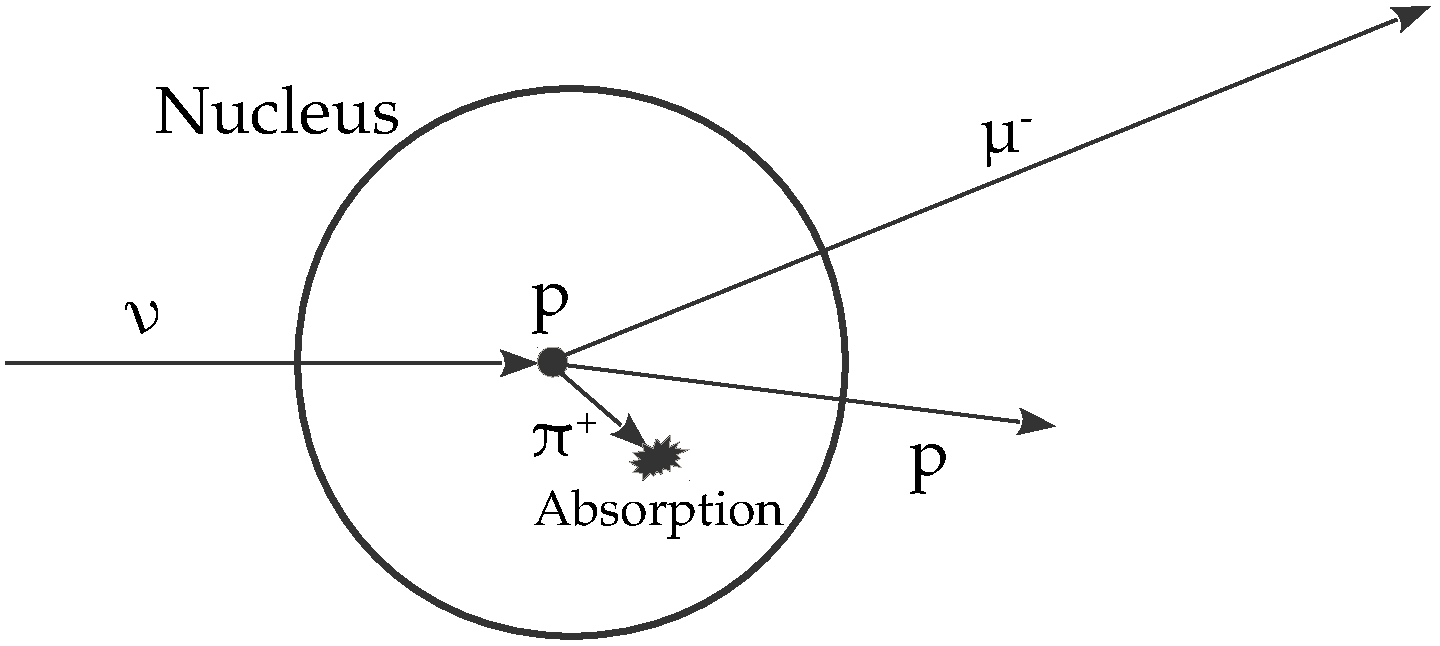
\includegraphics[width=.6\textwidth]{images/inter_nuc.pdf}
        \caption{A schematic of a potential interaction which may occur within the nucleus of an argon atom in SBND, leaving the pion invisible to the detector and the true interaction unidentifiable.}
        \label{fig:interNuc}
    \end{figure}

Another phenomenon that is not accounted for in the free nucleon theory is the potential for multiple nucleons to be involved in the intital scattering process. Such nucleons proceed to leave the nucleus and can appear to be products of an unphysical interaction such as the one in equation~(\ref{eq:fakeMEC}),

    \begin{equation}\label{eq:fakeMEC}
        p + \nu_{\mu} \longrightarrow p + p + \mu^{-}
    \end{equation}

    when infact, the interaction in equation~(\ref{eq:realMEC}),
    
    \begin{equation}\label{eq:realMEC}
        n + p + \nu_{\mu} \longrightarrow p + p + \mu^{-}
    \end{equation}

    actually occured within the nucleus, which is known as the 2-particle 2-hole effect, dominated by the Meson Exchange Current (MEC) \cite{MEC}.      \\

    In recent experiments, an excess of scattering events have been observed with respect to the theoretical predictions. It is now believed that MEC could be responsible, and it is therefore a primary concern of theorists, neutrino event generators and nuclear physicists to work together in correctly simulating what may occur in all future neutrino experiments with nuclear targets, in order to overcome these issues \cite{MEC}.

    The region of interest with respect to this excess of scattering events is depicted in Figure~\ref{fig:dipReg} \cite{dipReg}. The point of cross-over between the QE and Inelastic interaction cross sections alone dips significantly, whereas the data indicates that the dip should not be quite as drastic. When adding in the MEC contribution and calculating the total cross section, this dip region increases to fit more closely with the data.  

    \begin{figure}[h!]
        \centering
        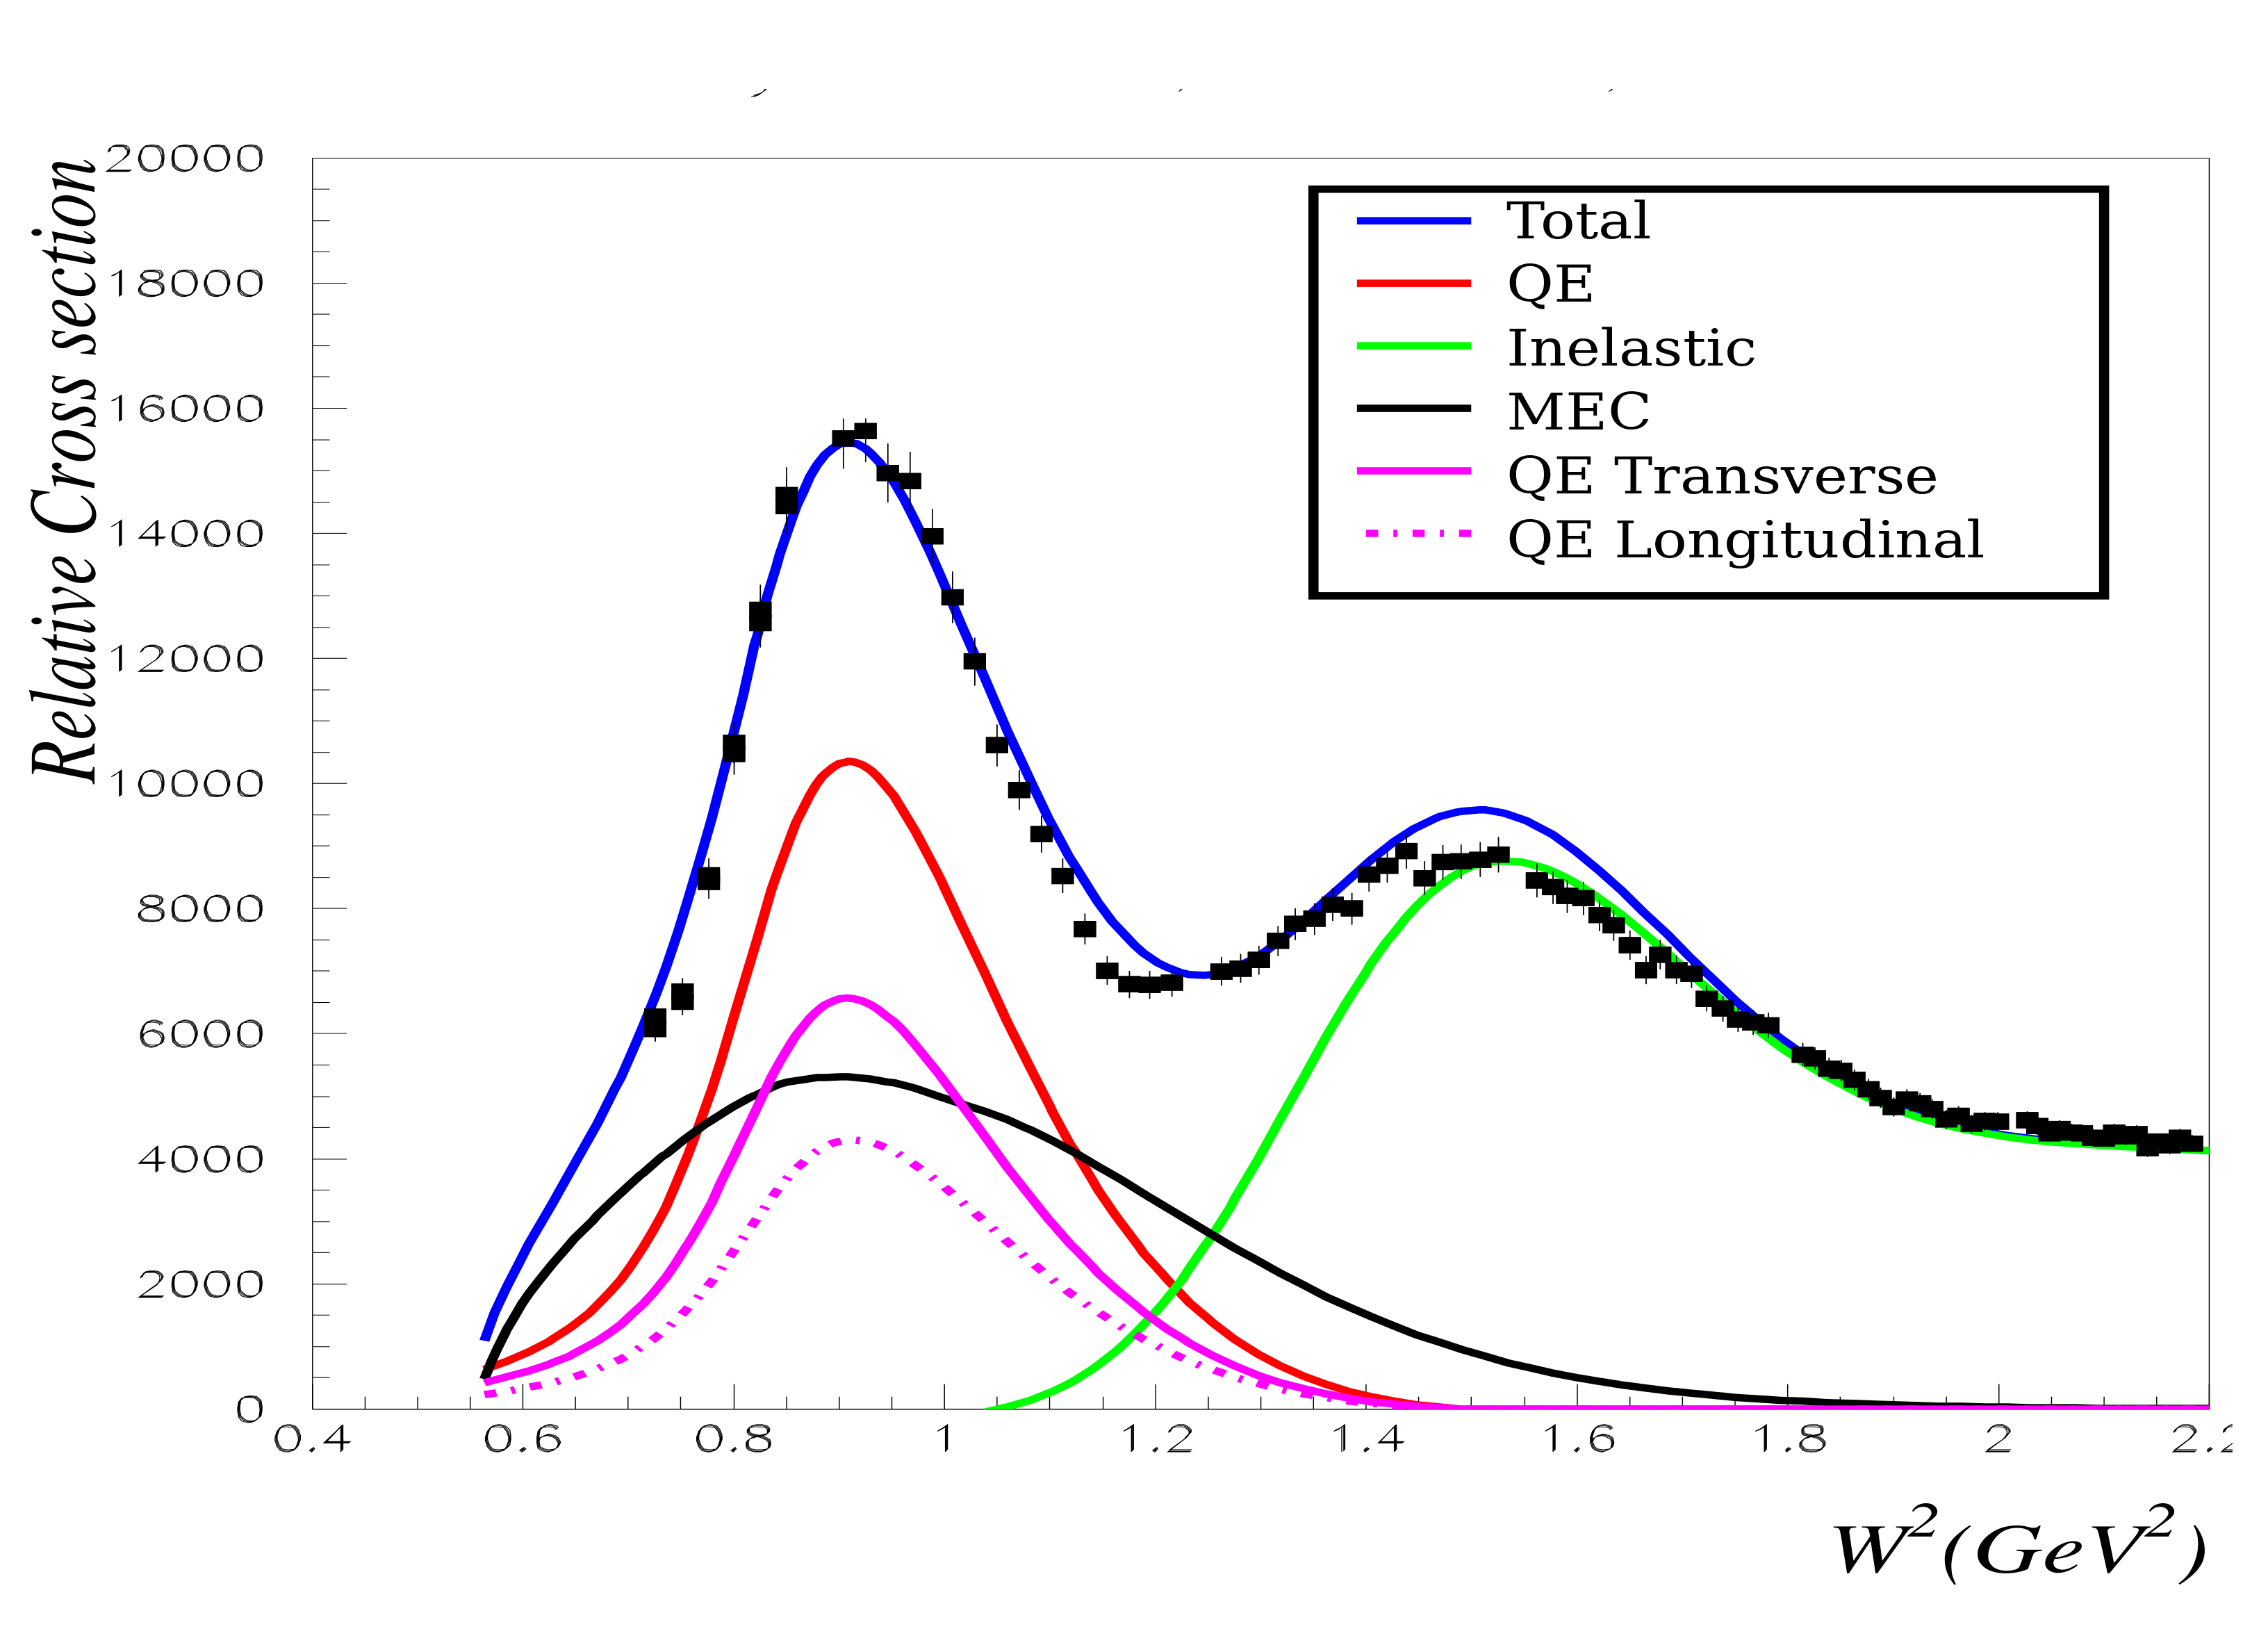
\includegraphics[width=.8\textwidth]{images/dip_region_3.png}
        \caption{The contribution of various interactions to cross section predictions, it is only with the inclusion of MEC that the total cross section comes close to resembling that of data}
        \label{fig:dipReg}
    \end{figure}

    Another indication that MEC is the cause of the observed excess is shown in Figure~\ref{fig:CCQEXsec} \cite{xsecModels}. In this diagram, various theoretical models are shown along with the data obtained. Here, most of the models fit to one another, but their cross sections collectively reside much lower than appears in the data. The closest fitting model to this data is the Martini, LFG+2p2h+RPA model, where 2p2h is the MEC contribution. Though tuning the parameter M\(_{A}\) also improves the RFG fit.  

    \begin{figure}[h!]
        \centering
        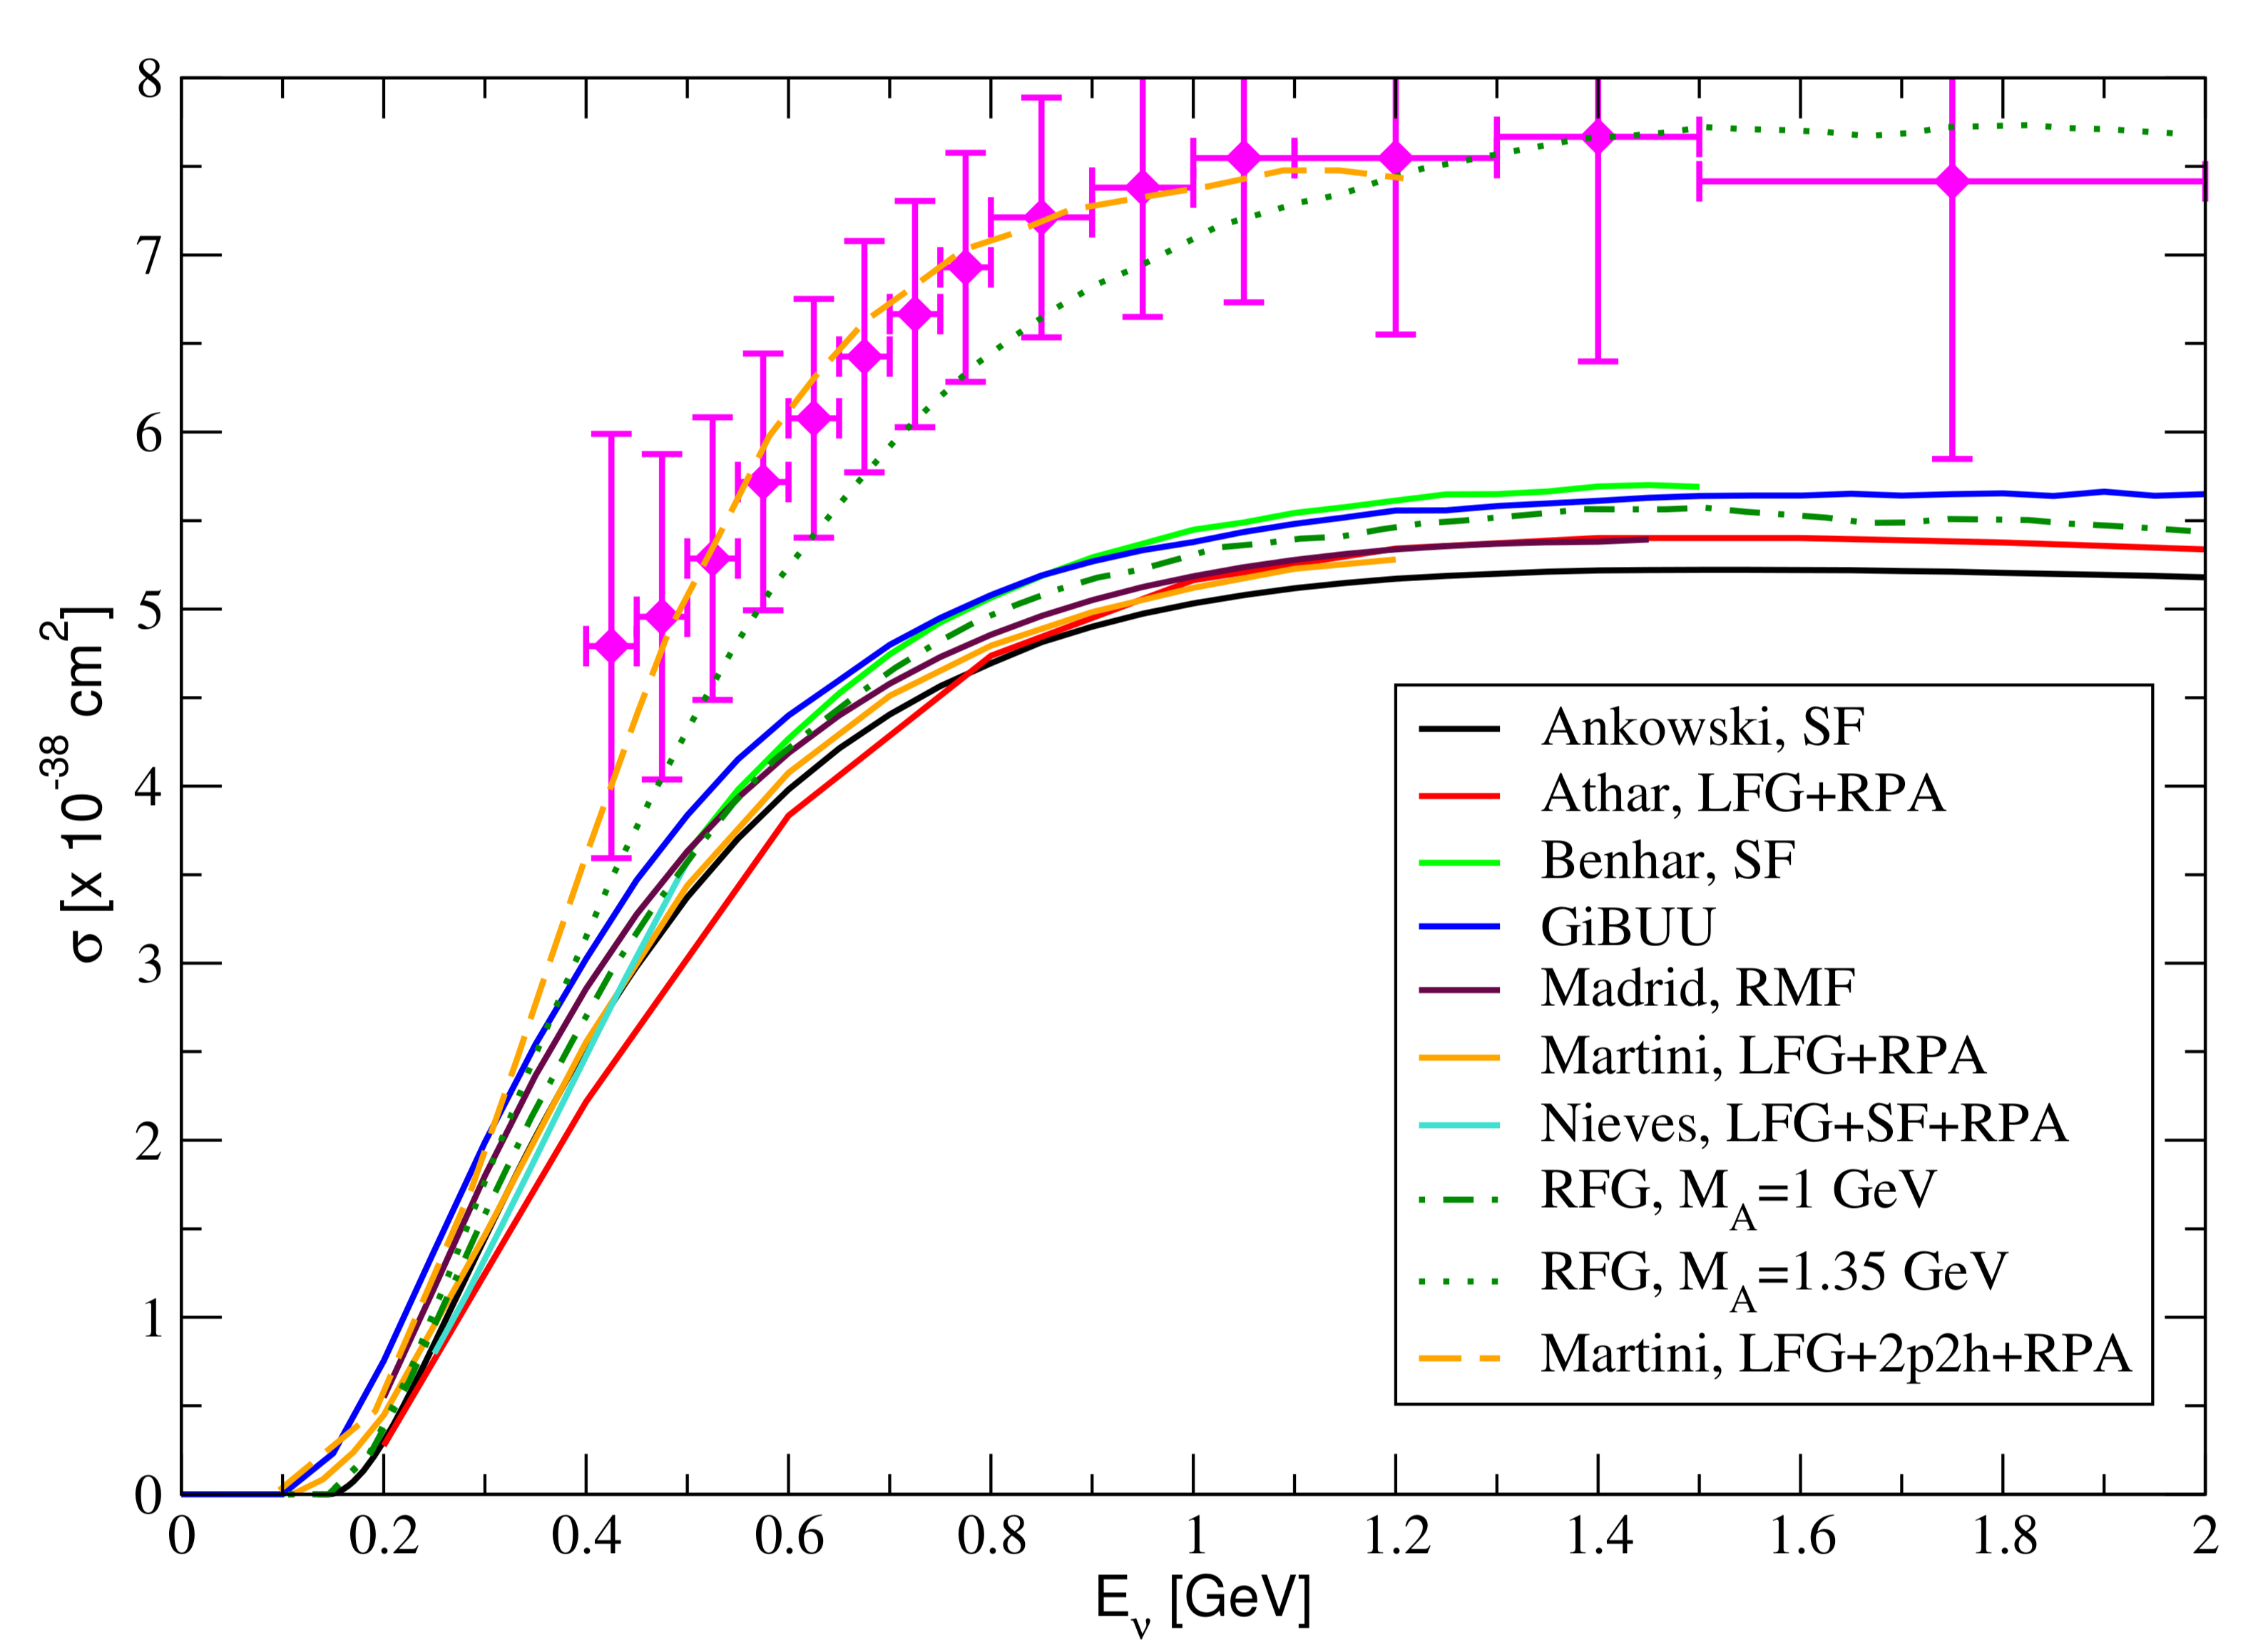
\includegraphics[width=.8\textwidth]{images/CCQE_xsec_2.png}
        \caption{A collection of theoretical predictions made for the CCQE interaction compared with data, once again it is a model with the contribution of MEC which comes closest to correctly predicting the trend of the data, though tuning M\(_{A}\) improves the fit of the RFG model.}
        \label{fig:CCQEXsec}
    \end{figure}

It is therefore clear that constructing model configurations with the correct physical theory is extremely important, but tuning the parameters which make up the models is also a crucial component in building predictions.

\clearpage


%---------------------------------------------------------------------------------------------------------------
\section{Theory and Recent Measurements of CC0\( \pi \) Cross-Section}
\label{sec:XSec}

\subsection{Cross-sections}
    % Plan
    \begin{itemize}

        \item Why?
        
        \begin{itemize}

            \item Simulation
            \item GENIE

        \end{itemize}
        
        \item Historical
        \item Current knowledge
        \item Needs for future
        
        \begin{itemize}

            \item LArTPCs
            \item Statistics

        \end{itemize}

    \end{itemize}

Inc. equations
\subsection{Method}
\subsection{Unfolding}
\subsection{Results}
Plots and cross-section values

\clearpage


%---------------------------------------------------------------------------------------------------------------
\section{A Global Fit of CC0\( \pi \) Data}
\label{sec:GF}

%Plan

\subsection{GENIE and the comparisons}
    GENIE applies theoretical physics models, composed of both physical and unphysical parameters, to detector geometries and materials to build experiment-specific neutrino interaction predictions. The collaboration is in the process of improving configurations of these models for the purpose of optimising the accuracy of the predictions.

    An archive of experimental data is publicly available, and provides the key ingredient to this configuration update. Comparing the models with these data sets allows for a direct performance evaluation of the predictions, whilst fitting the models to the data enables the parameters to be tuned and consequently improve the prediction.

The GENIE models are constructed as follows:

\begin{itemize}
    \item GENIE Model Tables
\end{itemize}

The model used in the tuning addresses the observation of the abnormalities seen in recent experiments by incorporating the MEC interaction, Figure~\ref{fig:MECSchem} describes this interaction schematically in terms of the models involved. 

\begin{figure}[h!]
    \centering
    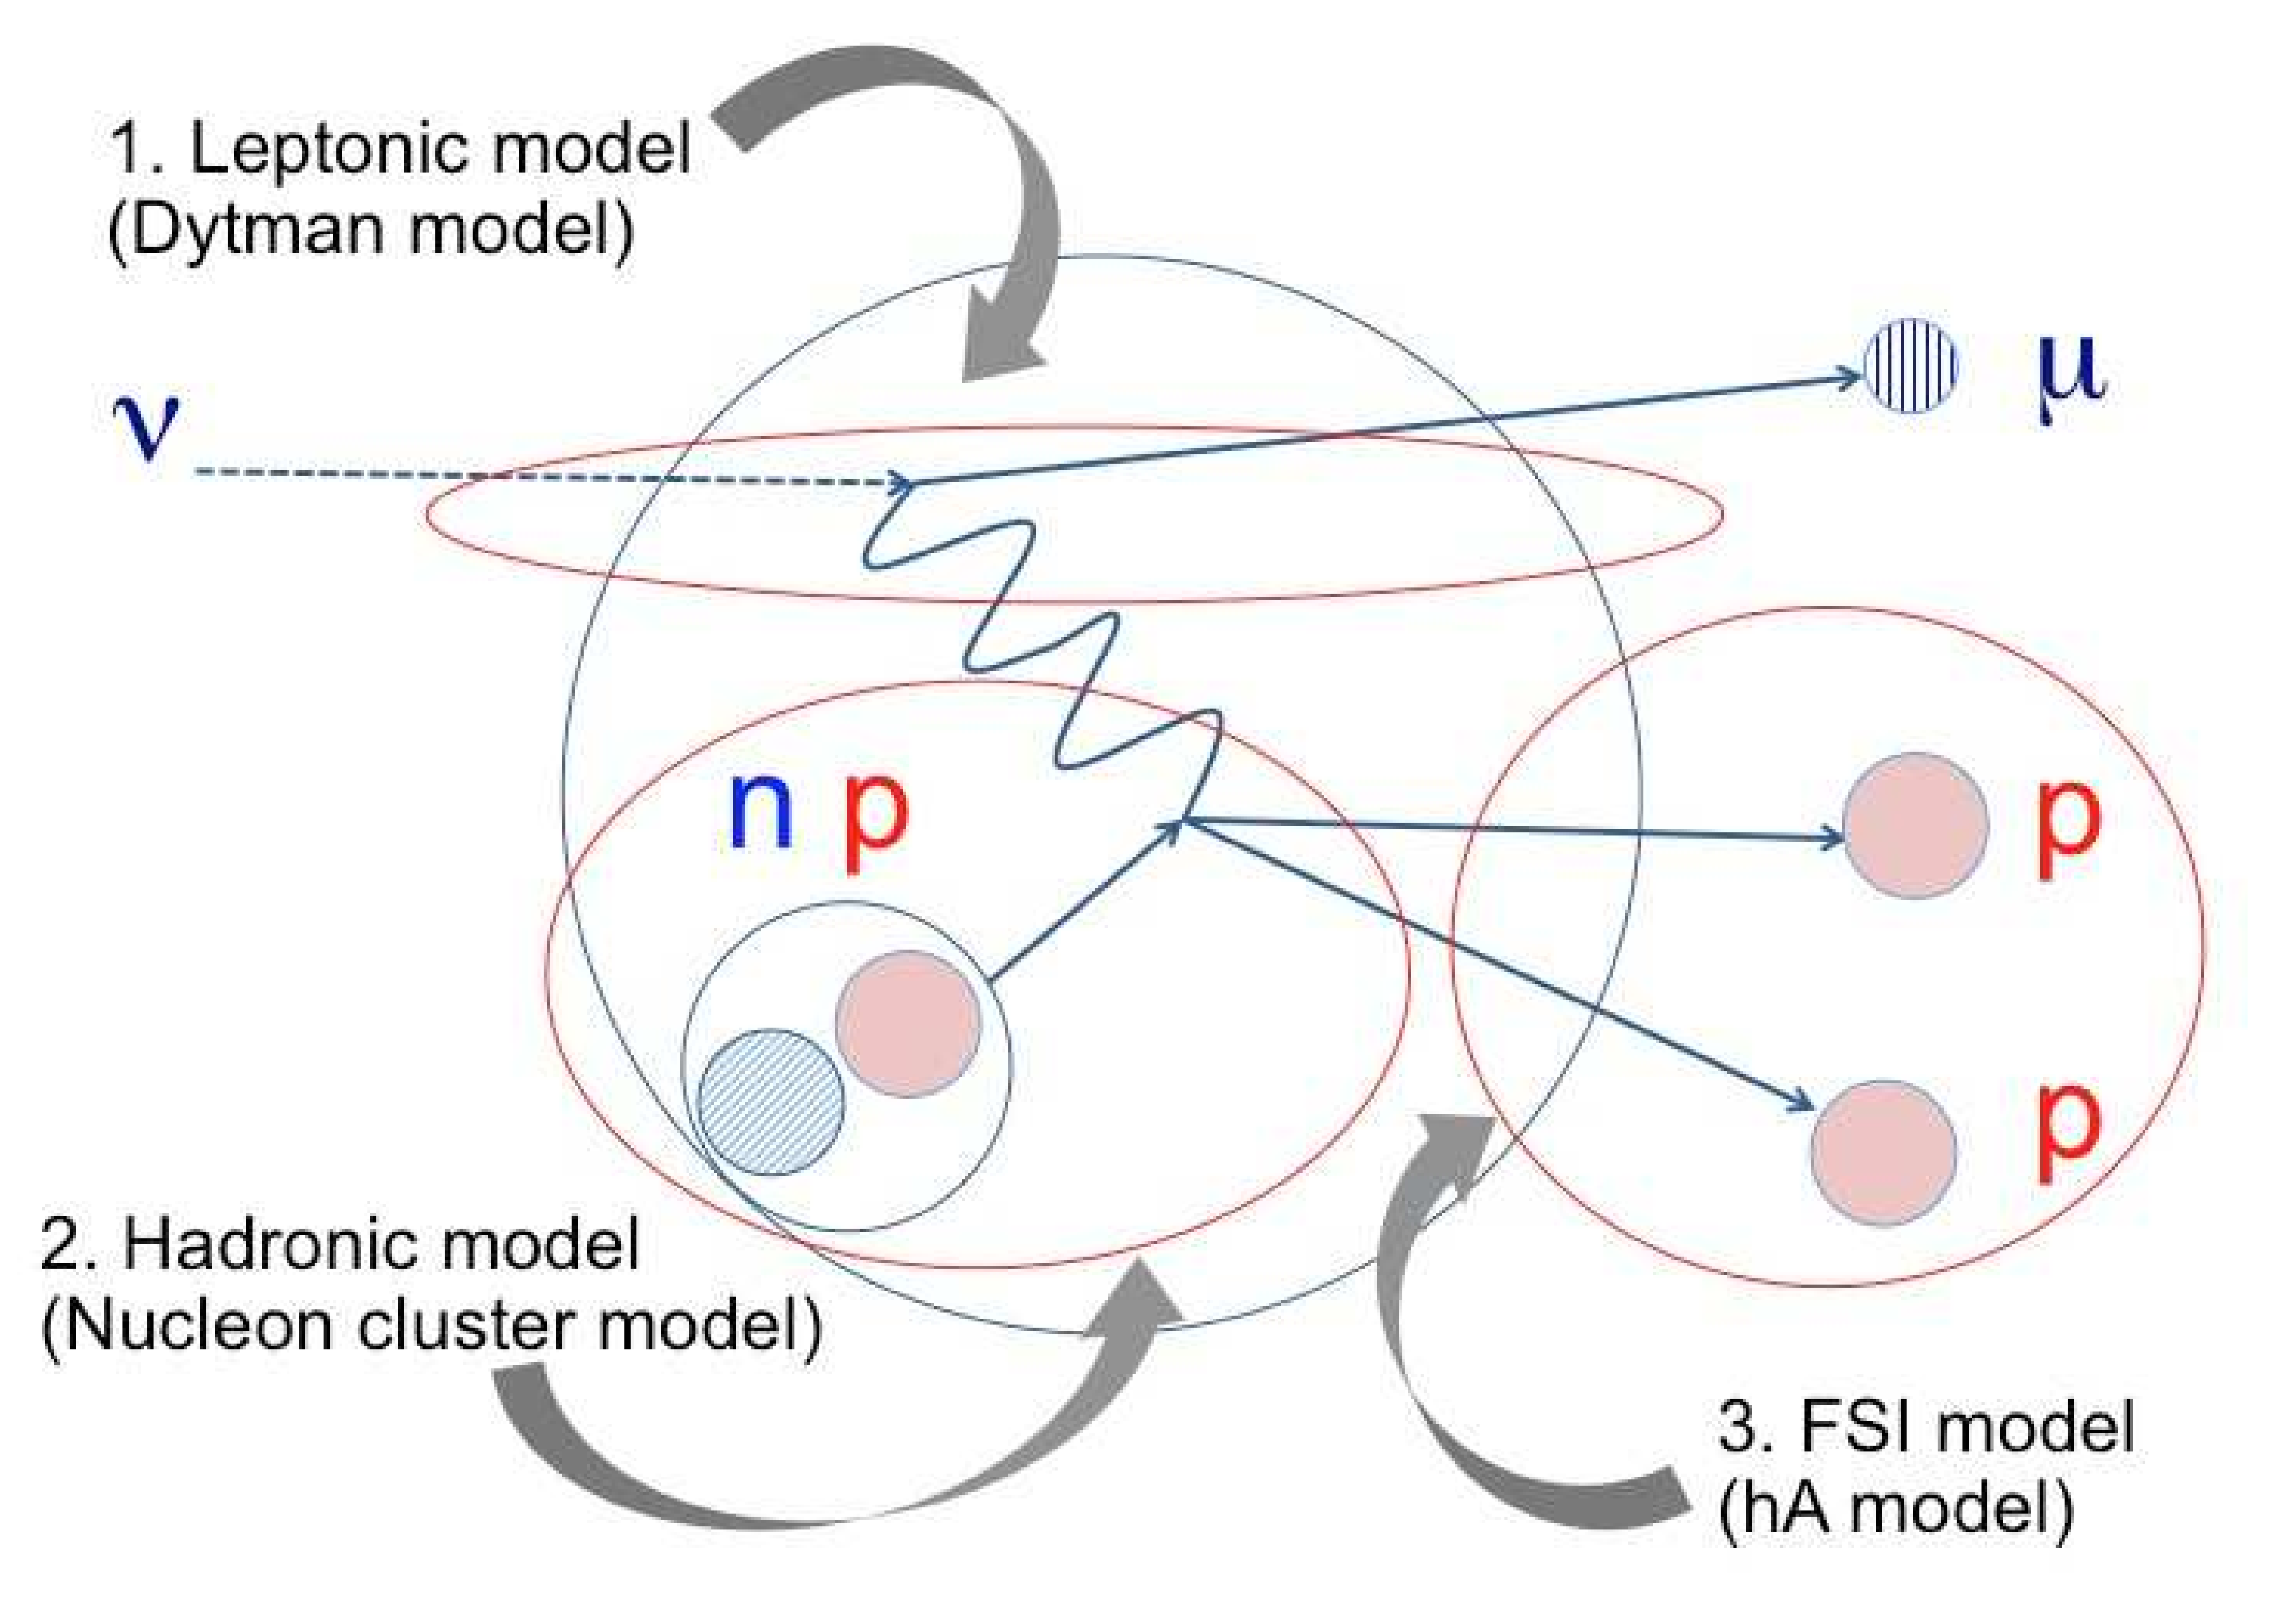
\includegraphics[width=.6\textwidth]{images/mec_model_genie.png}
    \caption{The models involved in the construction of the MEC model in neutrino event generation.}
    \label{fig:MECSchem}
\end{figure}

The incorporation of this model hopes to account of the ab


\begin{itemize}
    \item Publicly available datasets
    \item Comparisons
    \begin{itemize}
        \item MiniBooNE
        \item T2K
        \item Minerva
    \end{itemize}
    \item Tensions
\end{itemize}

\subsection{Process}
\begin{itemize}
    \item Motivate global fit
    \item Description of global fit
    \item Professor
    \begin{itemize}
        \item How it works
        \item Schematic
    \end{itemize}
\end{itemize}

\subsection{Results}
\begin{itemize}
    \item Results 
\end{itemize}



\clearpage


%---------------------------------------------------------------------------------------------------------------
\section{Prospects for a CC0\( \pi \) Measurement at SBND and Sensitivity Esimates}
\label{sec:Prospects}

\subsection{Discussion}
\subsection{SBND sensitivity}
\subsection{Conclusion and Future}

\clearpage


%---------------------------------------------------------------------------------------------------------------

\section{Discussion}


\clearpage


\newpage

%----------------------------------------------------------------------------------------
%	REFERENCE LIST
%----------------------------------------------------------------------------------------
\bibliographystyle{unsrt}
\bibliography{bib}

    %\bibitem{nuOsc} The Super Kamiokande Collaboration. Evidence for oscillation of atmospheric neutrinos. arXiv:hep-ex/9807003v2 31 Aug 1998.

    %\bibitem{nuInt} K. McFarland. Neutrino Interactions. arXiv:0804.3899v1 [hep-ex] 24 Apr 2008.
%---------------------------------------------------------------------------------------
\end{document}
